\chapter{Generazione dei video fake}

\section{Funzionamento}
\label{sec:funzionamento}

\section{Valutazione delle soluzioni disponibili}

Per la generazione dei video fake sono stati valutati tre applicativi diversi, forniti come Software-as-a-Service (SaaS):
\begin{itemize}
    \item DupDub.com
    \item Synthesia.io
    \item HeyGen.com
\end{itemize}

I criteri che sono stati valutati sono: la naturalezza dei movimenti generati, l'estensione dei movimenti generati, la qualità del lip-sync\footnote{sincronizzazione tra il movimento delle labbra di un soggetto e il suono delle parole pronunciate.}, la qualità e la naturalezza della voce parlata generata, e il grado di realismo generale dei video generati. Vediamo per ordine i punti di forza e di debolezza identificati di ognuno, e come si è pervenuti alla scelta finale. 

\subsection{DupDub}

DupDub si classifica come un prodotto "Talking-Photo". A partire da una fotografia di un persona, genera il movimento dei muscoli facciali e delle labbra per simulare il parlato. DupDub trova i suoi punti di forza nell'essere molto semplice, ma è stato valutato come troppo semplice per gli scopi di questa ricerca. La più grande limitazione è data dalla limitatezza dei movimenti, limitandosi appunto a generare solo movimenti dei muscoli facciali, e a malapena movimenti della testa, rendendo il risultato finale poco convincente e innaturale. Inoltre, tutti gli avatar forniti dalla piattaforma per la generazione dei video sono chiaramente soggetti non reali, generati a loro volta tramite IA.

\subsection{Synthesia.io}

Rispetto al precedente, Synthesia.io si mostra più capace. Fornisce avatar in mezzo busto, ed è in grado di generare movimenti del viso, della testa, e anche del corpo, producendo risultati più naturali di DupDub. Gli avatar forniti sembrano essere stati generati a partire da persone reali, ed il servizio offre la possibilità di generare avatar personali. I punti di debolezza individuati sono stati: la qualità del lip-sync e la qualità delle voci generate. In particolare, risultava frequente il disallineamento tra il movimento delle labbra dell'avatar e il suono della voce generato. La voce inoltre è stata valutata come poco espressiva e poco naturale. Vedremo in realtà come questi sono spesso i punti più deboli di questa tecnologia.

Nonostante questo, tale servizio poteva essere un buon candidato per la ricerca, ma è stato scartato a causa del piano offerto, in quanto offriva un servizio ad abbonamento basato su minuti. % Vi era un numero limitato di minuti di video generabili al mese, il che avrebbe limitato/rallentato il processo di ricerca.

\subsection{HeyGen}

Sin dal primo sguardo, HeyGen.com si è dimostrato essere al di sopra di tutti gli altri, offrendo la possibilità di generare video su sfondi reali, angolazioni diverse dello stesso avatar, e implementando movimenti del corpo avanzati come il movimento delle braccia e il gesticolamento delle mani. Gli avatar sono costruiti a partire da un video di riferimento di media durata del soggetto, il che li conferisce la possibilità di apprendere ed emulare i movimenti della persona inquadrata, producendo un risultato più naturale e realistico. Inoltre, la piattaforma si è dimostrata essere in constante evoluzione e sviluppo, arricchendo il suo catalogo di funzionalità, avatar e di voci durante il periodo di valutazione.

Per queste ragioni, tra le opzioni valutate, HeyGen è stato decretato come il migliore, in termini di qualità e naturalezza dei risultati prodotti, ed è stato quindi scelto come soluzione per la nostra ricerca. Un altro fattore che sicuramente ha giocato a suo favore è stato anche il piano offerto, il quale ci ha permesso di generare infiniti video durante il periodo di abbonamento, posto che questi fossero sotto i cinque minuti di durata.

\subsubsection{Profilo dei video fake}
Si delinea così il tipo di video che siamo in grado di generare: gli avatar sono privi di sfondo, per cui i video fake sono video raffiguranti una persona che parla, inquadrata a mezzo busto, con sfondo bianco, privi di movimenti di macchina o cambi di inquadrature, privi di animazioni o scritte che compaiono a corredo.

\section{Video real}

Identificata la piattaforma per la generazione dei video fake, è necessario procurarsi i video reali da utilizzare come riferimento per generare tali doppioni fake. Il tipo di video richiesto per i video real sono dei video brevi (durata inferiore ai 5 minuti), in modo che possano essere visionati per intero, e dai contenuti che non richiedano una particolare formazione pregressa per la loro comprensione, ma che non siano neanche banali, in modo di poter fare delle domande di comprensione a loro volta non banali. 

\subsection{Scelta dei video real}

\paragraph{Criterio di scelta}
È stata utilizzata per la ricerca dei video la piattaforma YouTube, e il criterio di ricerca dei video reali è semplice: cercare i video più simili possibili ai video fake che siamo in grado di generare. Per tali ragioni, il criterio di scelta consiste in video:
\begin{itemize}
    \item frontali, con un soggetto al centro su sfondo bianco
    \item con nessun movimento di macchina o cambi di inquadrature
    \item autodescrittivi, in altre parole non vengono utilizzate immagini, slide o grafici di supporto che vengono esplicitamente referenziati dallo speaker\footnote{questo perché contenuti esplicitamente referenziati dallo speaker reale non sarebbero presenti nel corrispettivo video fake, rompendo l'illusione.}
    \item con il minor numero di scritte o immagini che compaiono a corredo, preferibilmente nessuna
    \item con i sottotitoli preferibilmente inseriti a mano dall'autore del video, in modo da poter scaricare il copione associato al video più facilmente
\end{itemize}

\paragraph{Video trovati}

Per la realizzazione di un pilot della ricerca, sono stati identificati quattro video che soddisfano i criteri stabiliti:
\begin{itemize}
    \item \textit{"How to make a GREAT impression - Presentation Tips"} di Expert Academy %(https://youtu.be/lZg6H0WqPVY)
    \item \textit{"How to start a pitch or presentation"} di Dominic Colenso %(https://youtu.be/P2LwuF7zn9c)
    \item \textit{"How to start a presentation"} di Expert Academy %(https://youtu.be/LrjlW00kkws)
    \item \textit{"How to Get Over Your Fear of Public Speaking"} di Expert Academy %(https://youtu.be/So3Z93hEPDk)
\end{itemize}

I video sono stati scaricati utilizzando il tool open source \verb|yt-dlp| (\url{https://github.com/yt-dlp/yt-dlp}).

\subsection{Processing}

I video individuati non corrispondevano tutti perfettamente alle specifiche richieste, per cui per poterli integrare nella ricerca è stato necessario fare del pre-processing.

\subsubsection{Trimming}

Tutti i video individuati presentavano un introduzione e una coda al video, con musiche, scritte o elementi animati. I video individuati sono per cui stati tagliati, in modo da eliminare gli elementi non utili al nostro studio, e mantenere solamente la parte di video parlata. Per il trimming dei video è stato utilizzato il tool open source gratuito \verb|ffmpeg| (\url{https://www.ffmpeg.org}), così da favorire un'operazione veloce e priva di operazioni di re-econding ove possibile.

\subsubsection{Pulizia dello sfondo}

Alcuni dei video individuati presentavano alcuni elementi grafici a comparsa durante la parte parlata del video, come grafici o piccole scritte. Questo è stato valutato come accettabile visto che tali elementi non venivano referenziati esplicitamente dallo speaker, e comparivano solo in sovrapposizione dello sfondo.\footnote{Ricordiamo che tutti i video individuati presentano uno sfondo bianco uniforme, che non cambia nel tempo.} Questo ha permesso la rimozione di tali elementi aggiuntivi tramite una semplice operazione di video-editing, detta mascheramento.

\paragraph{Mascheramento}

Si identifica un fotogramma dell'immagine dove non vi sono elementi a coprire la parte dello sfondo interessata, e si salva tale fotogramma come file a parte. Questo fotogramma "pulito" è detto \textit{clean plate}. Dal momento che lo sfondo è statico, ovvero non cambia nel tempo, il clean plate funge da copia pulita dell'immagine, che possiamo utilizzare per coprire qualunque elemento in sovrapposizione dello sfondo. Con un qualunque programma di editing, si sovrappone il clean plate alla porzione temporale di video in cui compare l'elemento da rimuovere, ad esempio una scritta, e si effettua poi una maschera, che va a ritagliare il clean plate. Come una toppa, il clean plate mascherato copre il testo in sovra-impressione, rimuovendolo dal video. È possibile vedere un esempio di questa operazione in Figura \ref{fig:masking}.

\begin{figure}[ht]
    \centering
    \begin{subfigure}{0.32\textwidth}
        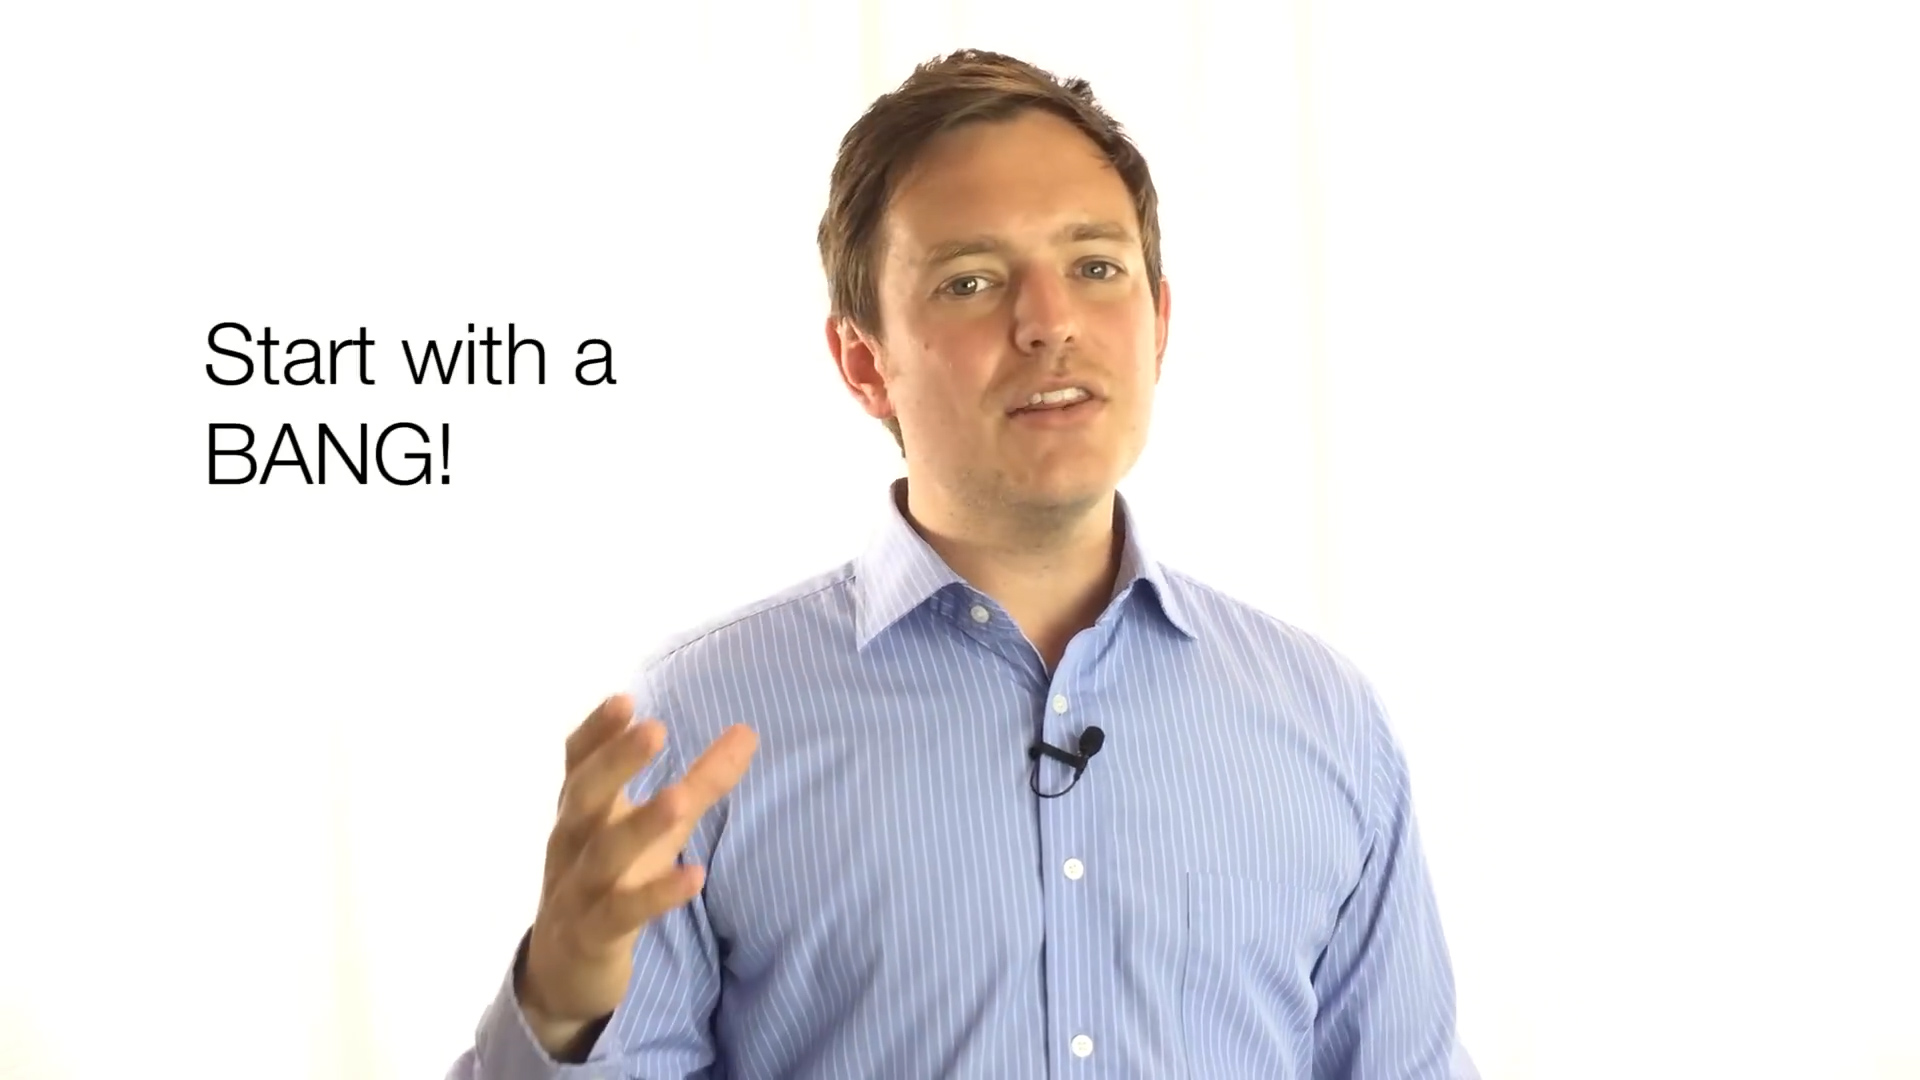
\includegraphics[width=0.95\linewidth]{images/original_frame} 
        \caption{Fotogramma originale}
        \label{fig:original_frame}
    \end{subfigure}
    \hfill
    \begin{subfigure}{0.32\textwidth}
        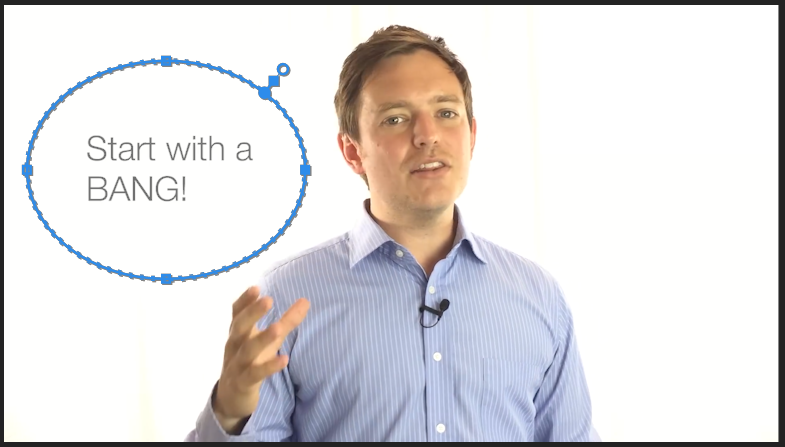
\includegraphics[width=0.95\linewidth]{images/mask_with_text}
        \caption{Maschera sovrapposta}
        \label{fig:mask_with_text}
    \end{subfigure}
    \hfill
    \begin{subfigure}{0.32\textwidth}
        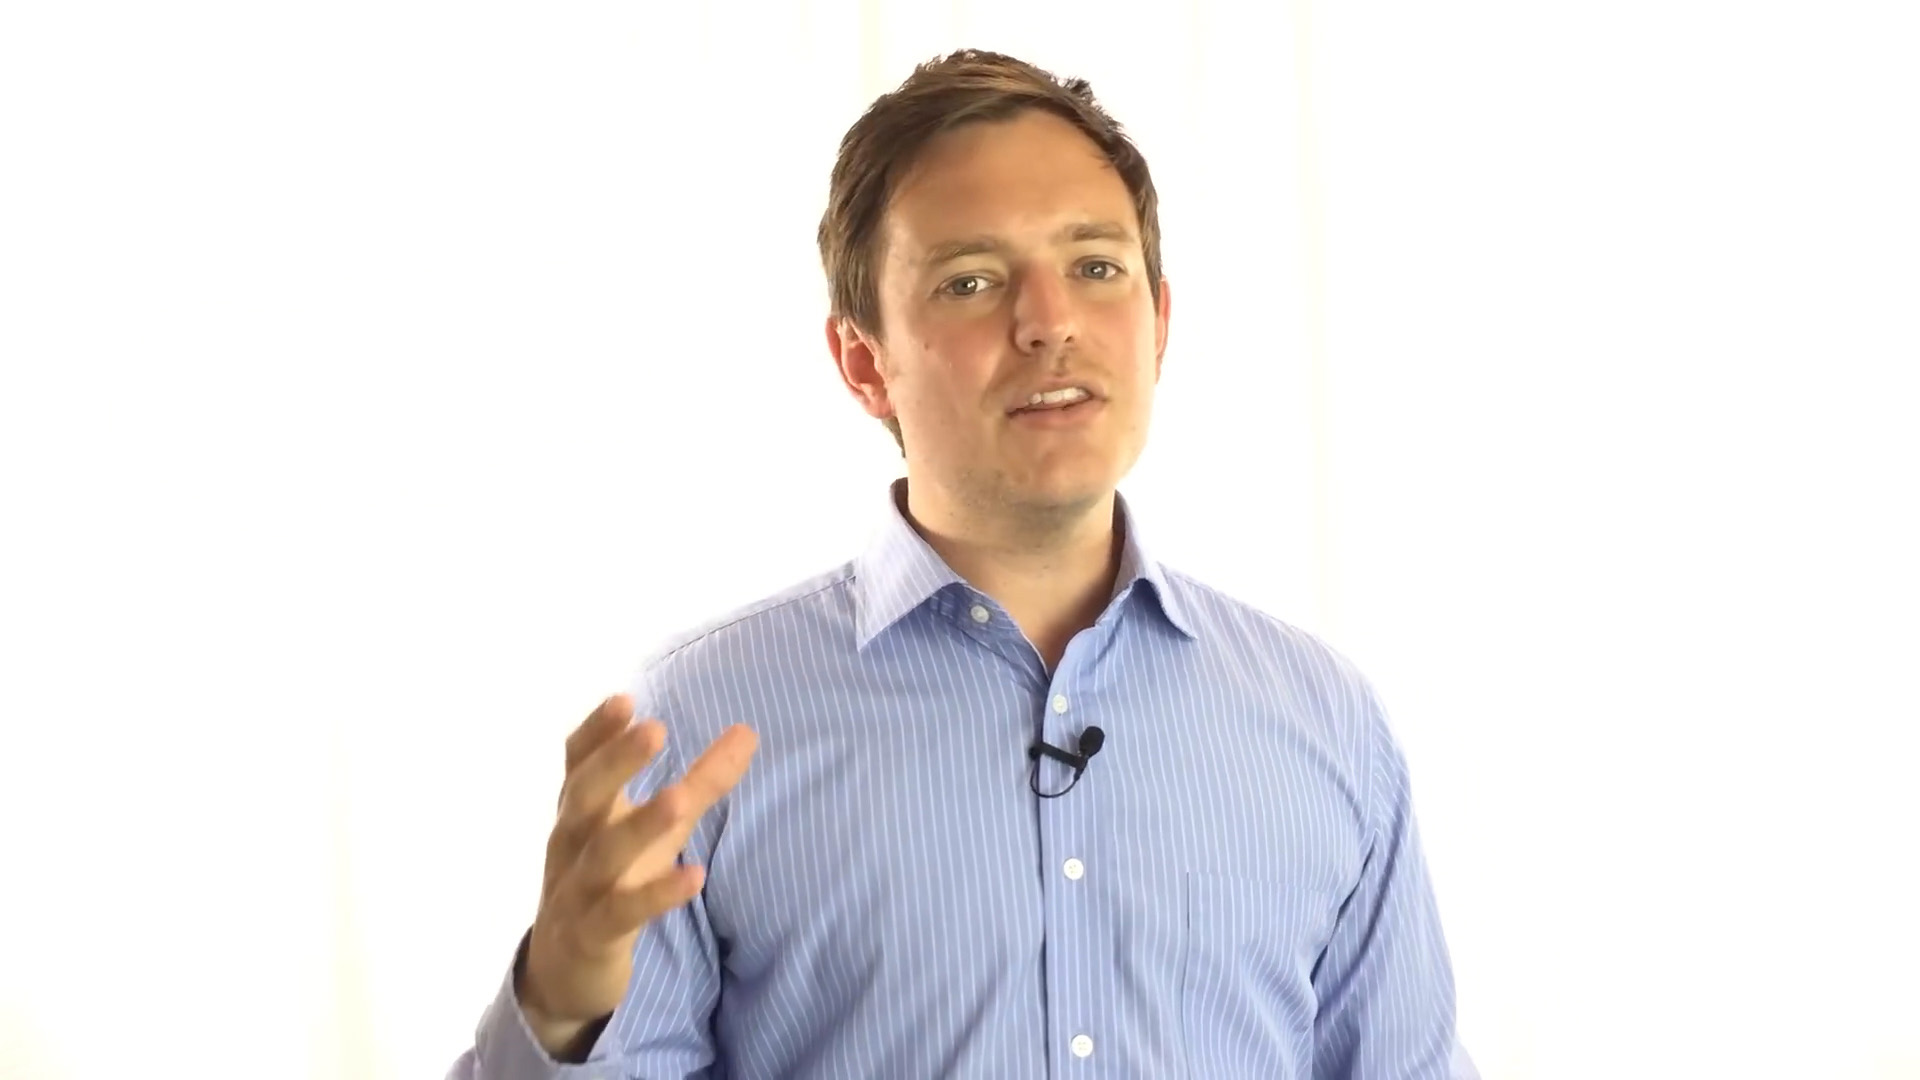
\includegraphics[width=0.95\linewidth]{images/masked}
        \caption{Fotogramma mascherato}
        \label{fig:masked}
    \end{subfigure}
    
    \caption{Una operazione di mascheramento con clean plate in Adobe Premiere Pro}
    \label{fig:masking}
\end{figure}

\subsubsection{Estrazione del testo}
\label{sec:text_extraction}

Per poter generare i doppioni fake, è stato estratto il testo associato al parlato presente nei video individuati. È stato utilizzato il sito web gratuito \url{https://downsub.com} per scaricare i sottotitoli già forniti da YouTube. La maggior parte dei video presentavano dei sottotitoli ufficiali, ovvero inseriti direttamente dagli autori dei video. Per gli altri, sono stati scaricati i sottotitoli generati automaticamente da YouTube, utilizzando quindi di fatto il motore SpeechToText integrato di YouTube.

In ogni caso, tutti i sottotitoli scaricati sono stati poi revisionati a mano per eliminare refusi, errori di battitura o di trascrizione, e per eliminare elementi non parlati o associati alle parti di video che sono state tagliate via. Questi file di sottotitolo sono tutto il necessario per generare i video fake.

\section{Generazione dei video fake}

Per la generazione dei video fake è stata utilizzata la piattaforma HeyGen (\url{https://www.heygen.com}). La piattaforma prevede la selezione di un avatar tra quelli forniti dalla piattaforma, la selezione di una voce tra i modelli TextToSpeech disponibili per generare il parlato, e infine l'inserimento del testo di riferimento.

Per ognuno dei video real individuati sono stati generati due video fake, uno con un avatar di genere maschile e uno con un avatar di genere femminile. Per la generazione di un video fake è stata seguita la seguente procedura, per ogni video real:

\begin{enumerate}
    \item Scelta di un avatar
    \item Scelta del modello di voce più adatto all'avatar scelto
    \item Se non è stata trovata una coppia avatar-voce convincente tornare al passo 1 passando al prossimo avatar
    \item Inserimento del testo estratto dal video real
    \item Fine-tuning del testo per migliorare intonazione, pronuncia e pause
    \item Revisione del risultato, ripetere il passo 5 se necessario
    \item Ripetizione del processo con un avatar del genere opposto
\end{enumerate}

% La procedura di generazione dei video fake ha previsto: la selezione degli avatar da utilizzare tra quelli forniti dalla piattaforma, la scelta della voce da utilizzare, ed eventuali modifiche del testo per migliorare la pronuncia o l'intonazione.

\subsection{Scelta degli avatar}

\begin{figure}[t]
    \centering
    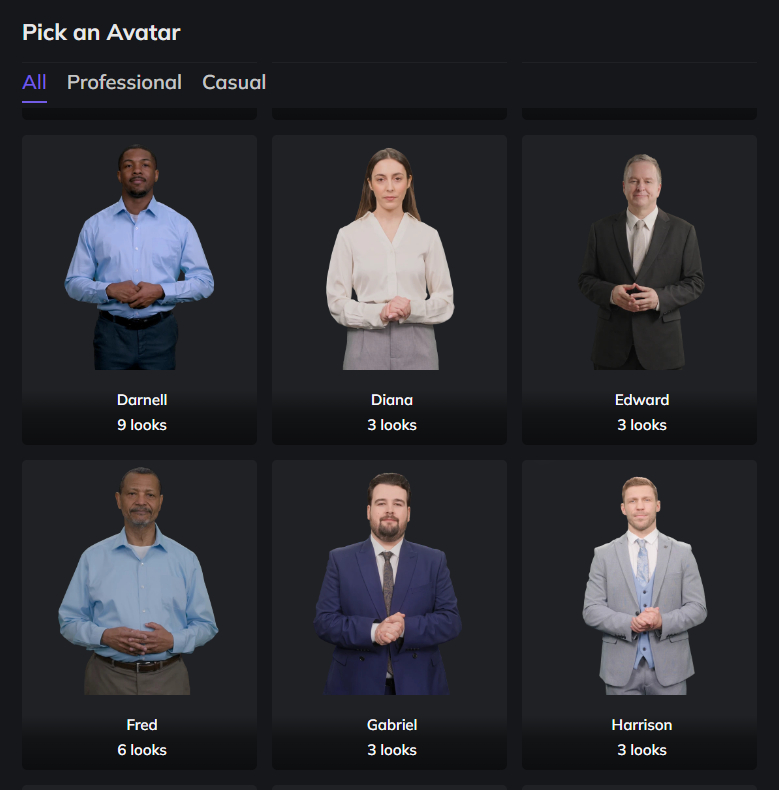
\includegraphics[width=0.62\linewidth]{images/pick_avatar}
    \caption{Esempio di schermata di selezione\\ dell'avatar della piattaforma HeyGen}
    \label{fig:pick_avatar}
\end{figure}

% \begin{figure}[t]
%     \centering
%     \includegraphics[width=0.9\linewidth]{images/heygen_platform}
%     \caption{La piattaforma di generazione HeyGen}
%     \label{fig:heygen}
% \end{figure}

Il punto di partenza per la generazione di un video fake è la scelta dell'avatar da utilizzare, ovvero la persona che verrà animata per realizzare il video parlato. La piattaforma HeyGen mette a disposizione una sua selezione di avatar proprietari, disponibili a tutti gli utenti del servizio, per realizzare i video fake. Gli avatar sono figure di persone a mezzo busto o in primo piano, prive di sfondo. È possibile vedere in Figura \ref{fig:pick_avatar} un esempio ridotto della schermata di selezione degli avatar forniti da HeyGen. Tra gli avatar sono disponibili look molto variegati, tra cui figure in abiti formali, completi, in camice, abiti da lavoro, abiti casual, etc. Per il nostro studio, sono stati considerati avatar con un look semi-formale o casual.

La piattaforma offre anche la possibilità di realizzare un proprio avatar, a propria immagine e somiglianza, ma non è stato possibile nel nostro studio usufruire di questa feature, avendo utilizzato come video real video di terzi.\footnote{È richiesto il consenso esplicito del soggetto rappresentato per realizzare un avatar a sua immagine.} 

% future works: ripetere l'esperimento realizzando video in casa, così da poter avere la stessa persona tra video real e fake

\subsection{Scelta delle voci}

\begin{figure}[t]
    \centering
    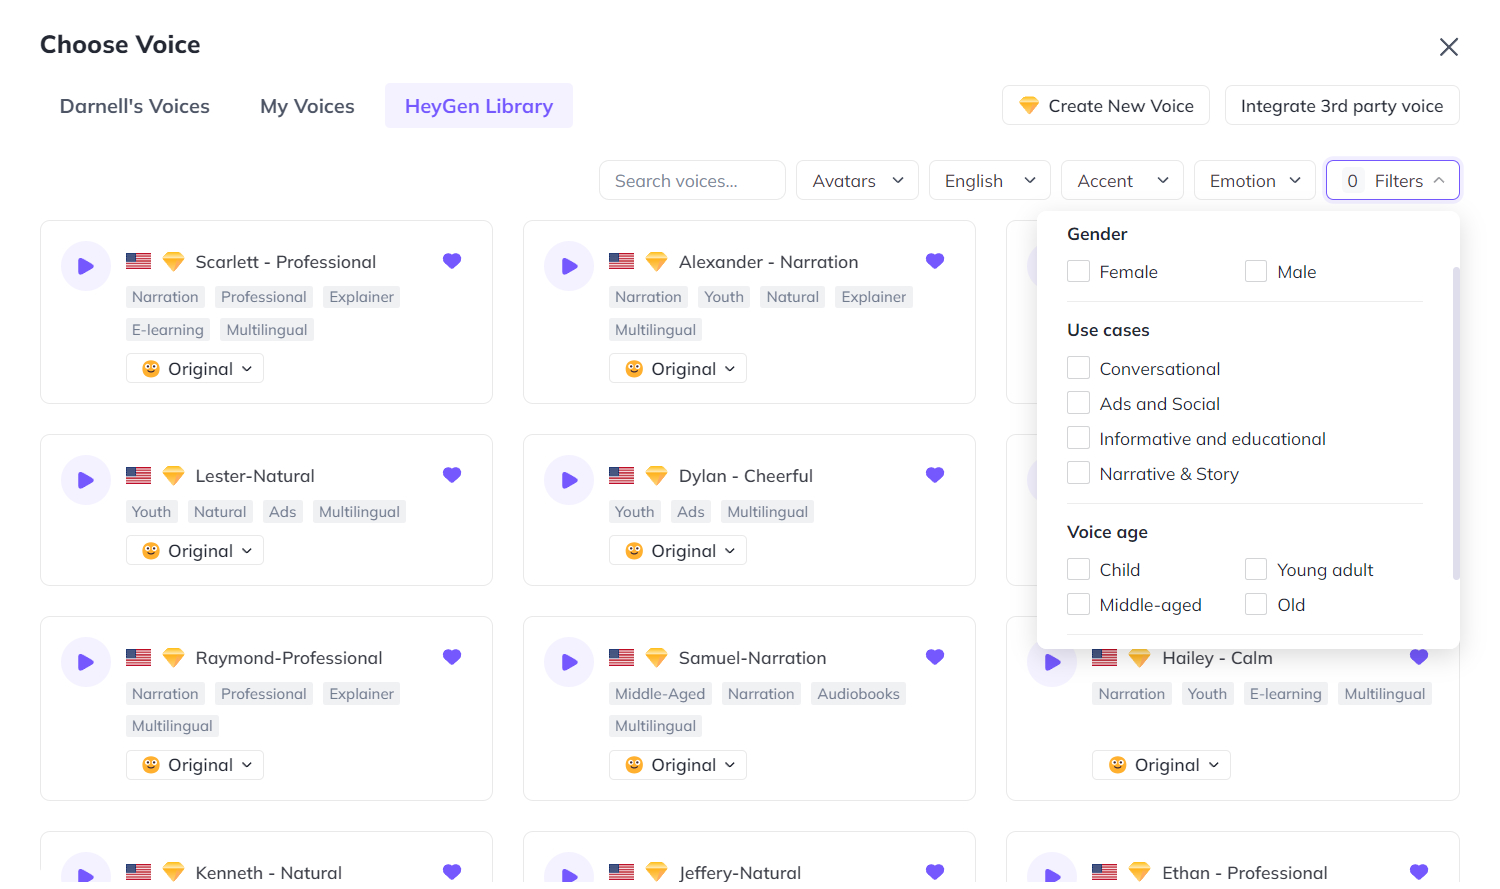
\includegraphics[width=0.9\linewidth]{images/voice_selection}
    \caption{Schermata di selezione della voce sulla piattaforma HeyGen.}
    \label{fig:voice_selection}
\end{figure}

Come anticipato, la scelta degli avatar non è stata fatta in modo indipendente, ma è stata fatta in funzione dei modelli di voce forniti dalla piattaforma HeyGen. Difatti, anche se il video generato è visivamente impeccabile, una voce innaturale o non calzante all'avatar selezionato è in grado di rompere completamente l'illusione, risultando chiaramente artificiale, o può essere un fattore di distrazione, in grado di impedire la fruizione normale del contenuto. Riconosciamo come il giudizio di una proprietà come una voce "calzante al soggetto identificato" può essere fortemente personale, così come anche fortemente umana, e meriterebbe uno studio approfondito a parte. Per i nostri scopi, la scelta è stata guidata dal giudizio umano. 

\subsubsection{Filtraggio tramite categorie di voci}

La piattaforma mette a disposizione un catalogo di voci molto variegato, suddiviso per categorie. Le categorie fornite sono visibili in Figura \ref{fig:voice_selection}, e sono: genere (Maschio, Femmina), età (Child, Young adult, Middle-aged, Old), e "use case" (Conversazionale, Pubblicità e social, Informativo ed educativo, Narrativo). Sono state innanzitutto filtrate le voci selezionando il genere appropriato e la fascia di età appropriata per l'avatar selezionato. In aggiunta, sono state favoreggiate voci categorizzate come a scopo "Informativo ed educativo", ma se necessario sono state valutate anche voci con altri use-case.

\subsubsection{Processo di selezione}

Isolate le possibili voci candidate, è stato generato un video per ogni voce. È stata selezionata poi, tra le candidate, la voce che, visionando il video generato, al giudizio umano è parsa più naturale e convincente con l'avatar selezionato. Se nessuna voce delle voci provate tra quelle fornite dalla piattaforma HeyGen è risultata convincente, l'avatar è stato scartato.\footnote{C'è da notare come con il tempo la piattaforma si è evoluta, e al tempo della scrittura di questo documento, HeyGen fornisce insieme agli avatar una pre-selezione di voci adatte all'avatar selezionato. Questo processo risulterebbe per cui molto semplificato.}

\subsubsection{Lingua} Tutti i video sono stati generati in lingua inglese poiché, sebbene HeyGen fornisca modelli di voci italiane, questi al tempo della ricerca erano limitati in numero e di qualità fortemente limitata rispetto alle controparti anglosassoni.

\subsection{Scrittura del testo}

\begin{figure}[t]
    \centering
    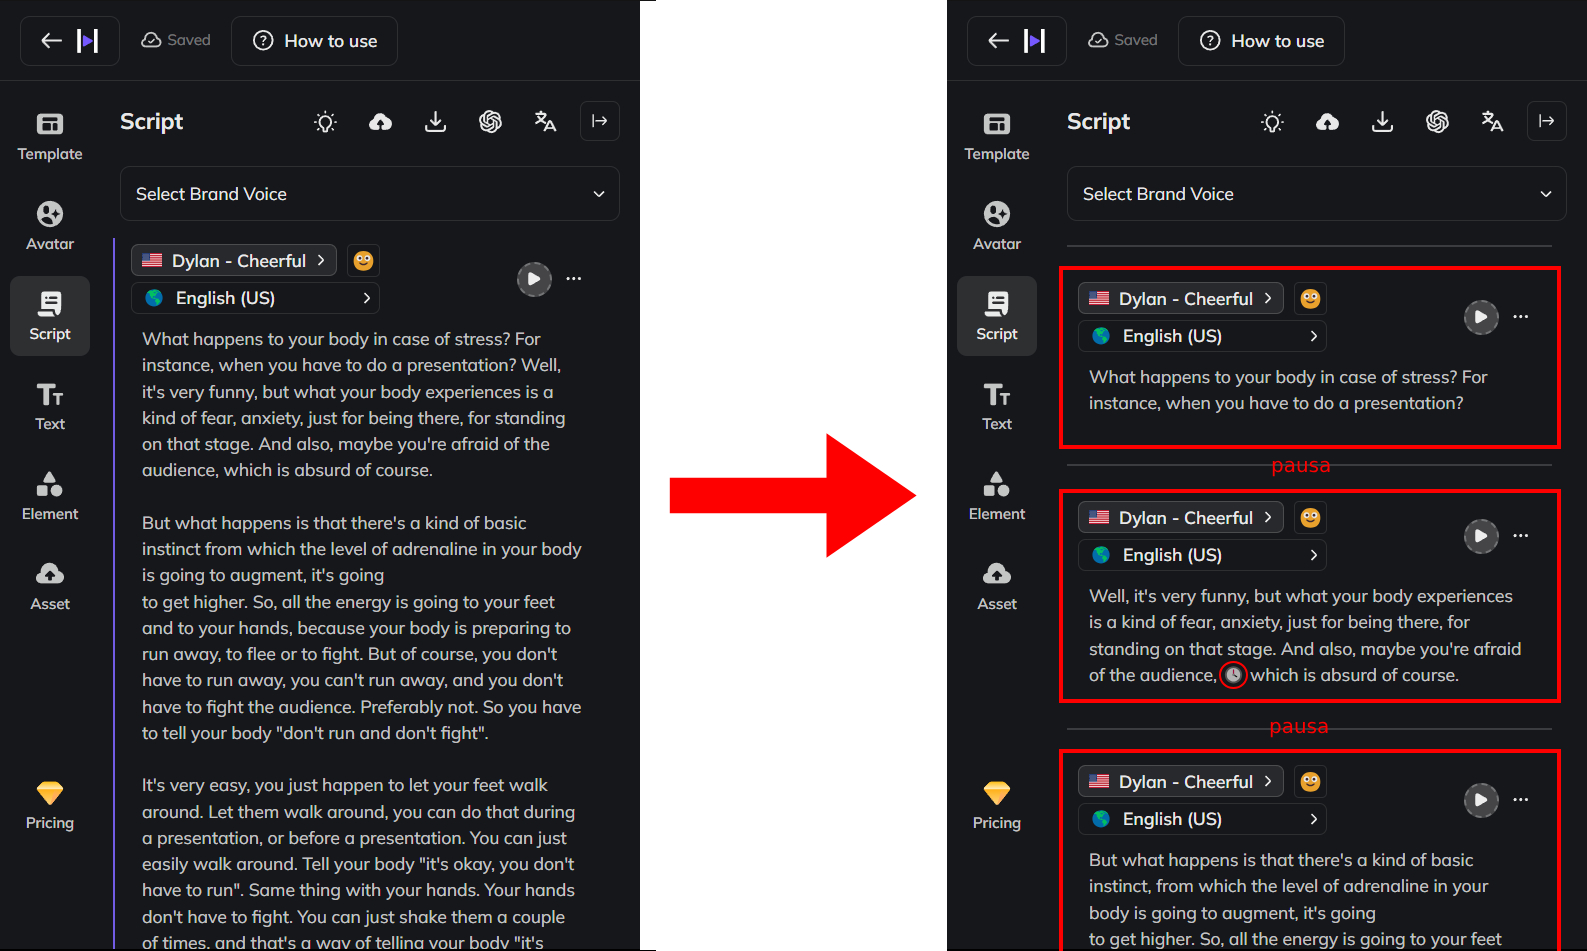
\includegraphics[width=0.9\linewidth]{images/text_heygen}
    \caption{Separazione del testo in paragrafi per introdurre pause naturali.}
    \label{fig:text_heygen}
\end{figure}

L'ultimo passaggio per generare un video fake è l'inserimento del testo da far esporre all'avatar. Nel nostro caso, si tratta del testo estratto dai video real, come spiegato in \ref{sec:text_extraction}. 
I punti chiave di questo passaggio sono: l'introduzione di pause per un flusso naturale del discorso, e la specifica di particolari pronunce, ove necessario.

\subsubsection{Introduzione di pause}
    
La piattaforma HeyGen permette di introdurre pause nel discorso in modo naturale separando il testo in "paragrafi". I paragrafi sono blocchi indipendenti di testo a partire dai quali è generata la voce. Tra un paragrafo e l'altro viene inserita automaticamente una piccola pausa, permettendo un flusso naturale del discorso. È possibile vedere un esempio di separazione in paragrafi in Figura \ref{fig:text_heygen}.

\subsubsection{Revisione del risultato}

A partire dal testo inserito viene generato l'audio della voce, che farà da guida per la generazione dei movimenti dell'avatar, come spiegato in \ref{sec:funzionamento}. Prima di avviare la generazione del video è possibile generare un'anteprima della voce. Se non si identificano problemi di pausa o di pronuncia, si fa partire la generazione del video.

\subsection{Download dei risultati}

Una volta generati i video, questi sono visualizzabili sulla piattaforma e scaricabili gratuitamente in formato 720p o 1080p.

\clearpage